\begin{figure*}[t]
\centering
% Vector drawing generated by tools/figures/architecture.py; rerun it after changing the figure.
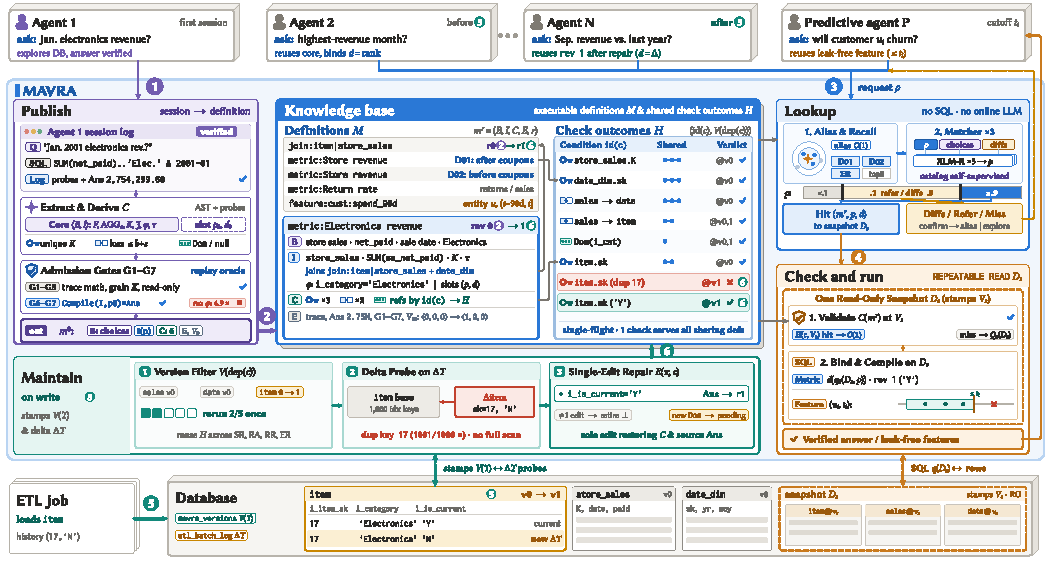
\includegraphics[width=\textwidth,trim=0 0.2mm 0 0.6mm,clip]{figures/architecture}%
\caption{\bt{Components of \system{} around one shared knowledge base, and the path of one definition through them: publication (steps 1--2), lookup and reuse (3--4), and maintenance after a write (5--6). Small circled numbers mark the step that wrote a state.}{\system{} 围绕一个共享知识库的各组件，以及一个定义经过它们的路径：发布（步骤 1--2）、查找与复用（3--4）、写入后的维护（5--6）。小圆圈数字标出写入该状态的步骤。}}
\label{fig:architecture}
\Description{Agents 1, 2, N and predictive agent P sit above MAVRA; the database and an ETL job sit below it. Inside MAVRA, five components surround a knowledge base. Publish, on the left, takes Agent 1's verified session (the SQL with the filter i_category = 'Electronics' marked as phi and the period d_year = 2001 AND d_moy = 1 marked as parameter p, the probes, and the answer 2,754,299.60), extracts the implementation I and parameter p0 with an LLM, derives conditions C (keys unique, join coverage within b plus epsilon, domain and null bounds from probes) without an LLM, and passes gates G1 to G7; replaying on the learning tables shows that Compile(I, p0) equals the answer while a draft without phi is 4.9 times larger and is rejected. Its output, revision 0, enters the knowledge base (step 2). The knowledge base is one key-value store shared by all agents. Definitions are entries keyed by kind and name, one per revision m^r = (B, I, C, E, r): join:item|store_sales, two metric:Store revenue entries (D01 after coupons, D02 before coupons), metric:Return rate, feature:customer:spend_90d, and the expanded metric:Electronics revenue, whose joins reference the join entry by key and whose conditions reference outcomes in H by signature. The lookup state holds aliases (store turnover maps to D01 and D02), one vector per entry, and three judges trained on the catalog. Check outcomes H are keyed by (id(c), V(dep(c))): date_dim at version 0 passes and serves three definitions; store_sales to date_dim at version 0 passes; item at version 0 passes; item at version 1 fails and item with 'Y' at version 1 passes, both written in step 6. Lookup, on the right, receives requests (step 3), reads the alias table, recalls the 8 nearest definitions with bge-m3, scores them with three cross-encoder judges, and decides with thresholds 0.1 and 0.9; replies are hit, same name with differences, refer (a confirmed reference becomes an alias), or miss. A hit with m, p, d goes to Check and run (step 4), which checks C against outcomes in H at the snapshot's versions, runs the compiled query in one snapshot, compiles features per entity and cutoff, and returns the answer to the agent. At the bottom, the ETL job loads an item history row for key 17 (step 5). Maintain stamps versions V(T), Stage 1 skips conditions whose tables kept their versions and reruns 2 of 5 checks once for all definitions, Stage 2 checks only the inserted rows and finds key 17 twice, and Repair keeps a sole single edit that preserves the answer, i_is_current = 'Y', publishing revision 1 with outcomes at the new versions (step 6); otherwise it retires the definition or marks it pending. Thin arrows are calls, thick arrows write shared state, grey arrows are references by key or reads of the knowledge base, and dashed arrows read database state.}
\end{figure*}
